\cotefile{81}

\scanpage{12}
\figure{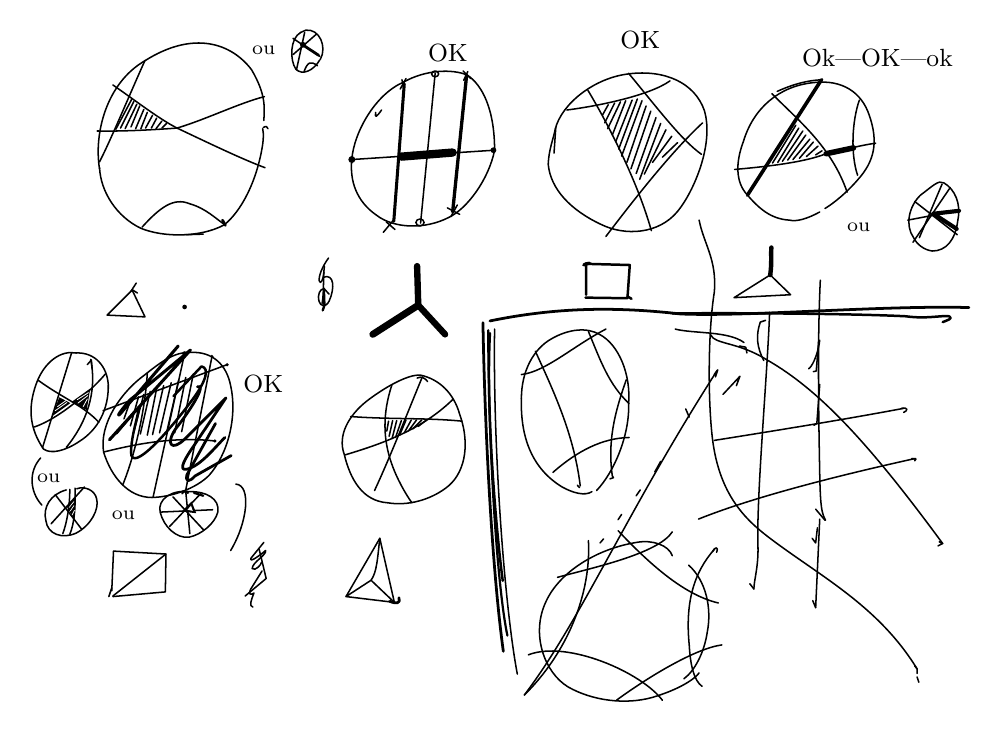
\begin{tikzpicture}[x=0.0074cm,y=-0.0074cm,line width=.55pt,line join=round,line cap=round,font=\small]
\begin{scope}
\draw (154,263) .. controls (144,202) and (166,116) .. (231,78)
 .. controls (316,24) and (381,48) .. (415,93)
 .. controls (440,136) and (437,157) .. (436,180);
\draw (434,194) .. controls (436,203) and (435,213) .. (434,221)
 .. controls (424,286) and (396,337) .. (368,359);
\draw (154,261) .. controls (156,302) and (183,345) .. (225,365)
 .. controls (264,381) and (328,381) .. (368,359);
\draw (302,376) -- (332,375);
\draw (435,192) .. controls (440,189) and (442,190) .. (443,194);
\draw (177,119) .. controls (220,149) and (256,177) .. (287,193)
 .. controls (342,219) and (398,246) .. (438,261);
\draw (232,77) .. controls (208,130) and (174,212) .. (154,251);
\draw (150,198) .. controls (202,199) and (259,195) .. (287,193)
 .. controls (337,178) and (394,150) .. (437,139);
\draw (227,363) .. controls (257,330) and (281,311) .. (309,323)
 .. controls (337,331) and (354,349) .. (368,358);
\draw[line width=1pt] (365,351) -- (370,360);
\draw (209,144) -- (182,195) (213,147) -- (190,193)
 (218,152) -- (198,194) (223,155) -- (208,191)
 (230,161) -- (216,194) (236,166) -- (225,194)
 (245,171) -- (233,193) (252,176) -- (243,193)
 (261,181) -- (251,194) (269,185) -- (261,193);
\node[inner sep=0pt,font=\scriptsize] at (436,59) {ou};
\draw (499,29) .. controls (481,39) and (480,76) .. (491,92)
 .. controls (502,103) and (521,95) .. (532,76);
\draw (533,75) .. controls (545,53) and (531,22) .. (508,25) -- (499,29);
\draw (506,29) -- (492,93);
\draw (486,39) -- (532,70);
\draw (486,67) -- (526,32);
\draw (505,96) .. controls (511,80) and (516,77) .. (528,86);
\fill (503,50) circle[radius=5];
\draw[line width=1pt] (504,51) -- (530,68);
\end{scope}
\begin{scope}
\draw (587,246) .. controls (591,200) and (627,135) .. (676,114)
 .. controls (713,93) and (759,91) .. (785,102)
 .. controls (811,119) and (832,161) .. (832,231)
 .. controls (822,281) and (785,331) .. (754,346)
 .. controls (712,368) and (659,365) .. (630,343)
 .. controls (595,319) and (583,284) .. (587,246);
\draw (587,247) -- (831,231);
\draw[line width=1.1pt] (677,117) -- (659,353);
\draw (730,99) -- (705,356);
\draw[line width=1.2pt] (784,102) -- (760,337);
\draw[line width=3pt] (672,242) -- (760,235);
\fill (587,247) circle[radius=6];
\fill (830,231) circle[radius=5];
\draw (730,100) ellipse[x radius=6,y radius=5];
\draw (704,355) ellipse[x radius=7,y radius=6];
\draw (673,110) -- (677,126) (680,108) -- (670,126);
\draw (778,95) -- (791,108) (786,96) -- (779,111);
\draw (646,354) -- (661,367) (660,349) -- (641,372);
\draw (751,330) -- (772,341) (768,325) -- (757,345);
\draw (638,162) .. controls (629,175) and (626,176) .. (628,166);
\node[inner sep=0pt] at (752,64) {OK};
\end{scope}
\begin{scope}
\draw (936,195) .. controls (947,151) and (1003,107) .. (1062,100)
 .. controls (1125,92) and (1176,116) .. (1192,163)
 .. controls (1209,220) and (1174,302) .. (1146,336)
 .. controls (1114,375) and (1056,379) .. (1014,358)
 .. controls (963,334) and (928,298) .. (924,255)
 .. controls (925,229) and (934,208) .. (936,195);
\draw (937,192) -- (934,236);
\draw (956,162) .. controls (1011,155) and (1098,137) .. (1133,112);
\draw (992,128) .. controls (1017,169) and (1075,276) .. (1101,369);
\draw (1062,99) .. controls (1110,157) and (1153,214) .. (1187,238);
\draw (1189,184) .. controls (1137,232) and (1074,312) .. (1023,379);
\draw (1027,153) -- (1017,171) (1038,150) -- (1021,184)
 (1048,148) -- (1026,194) (1057,146) -- (1034,205)
 (1068,145) -- (1040,216) (1077,143) -- (1045,229)
 (1085,146) -- (1050,241) (1092,155) -- (1059,252)
 (1100,164) -- (1066,263) (1109,175) -- (1075,271)
 (1117,185) -- (1081,281) (1126,196) -- (1089,272)
 (1136,207) -- (1103,252) (1146,218) -- (1120,243);
\node[inner sep=0pt] at (1082,42) {OK};
\end{scope}
\begin{scope}
\draw (1265,307) .. controls (1246,286) and (1245,253) .. (1259,216)
 .. controls (1276,159) and (1320,121) .. (1379,115)
 .. controls (1429,109) and (1462,132) .. (1475,171)
 .. controls (1491,217) and (1484,250) .. (1455,282)
 .. controls (1436,304) and (1414,322) .. (1399,331);
\draw (1390,337) .. controls (1368,349) and (1350,354) .. (1338,351)
 .. controls (1305,349) and (1285,330) .. (1265,307);
\draw (1317,130) .. controls (1344,118) and (1368,111) .. (1395,110);
\draw[line width=1.3pt] (1266,308) -- (1393,110);
\draw (1308,134) .. controls (1351,178) and (1410,224) .. (1437,303);
\draw (1244,264) .. controls (1300,259) and (1363,252) .. (1401,237)
 .. controls (1434,230) and (1462,222) .. (1486,219);
\draw[line width=2pt] (1401,237) -- (1448,227);
\draw (1458,145) .. controls (1445,182) and (1443,239) .. (1455,274);
\draw (1344,185) -- (1301,252) (1349,188) -- (1309,253)
 (1354,193) -- (1318,252) (1361,198) -- (1326,250)
 (1366,205) -- (1335,248) (1373,212) -- (1344,247)
 (1379,217) -- (1355,245) (1387,224) -- (1367,242)
 (1394,232) -- (1383,239);
\node[inner sep=0pt] at (1489,72) {\unsure{Ok|OK|ok}};
\node[inner sep=0pt,font=\scriptsize] at (1457,364) {ou};
\draw (1551,381) .. controls (1536,360) and (1543,327) .. (1563,308)
 .. controls (1582,294) and (1594,281) .. (1603,287)
 .. controls (1622,298) and (1633,323) .. (1627,351)
 .. controls (1623,385) and (1607,404) .. (1583,404)
 .. controls (1569,402) and (1557,393) .. (1551,381);
\draw (1553,319) -- (1626,376);
\draw (1541,351) -- (1630,334);
\draw (1550,389) -- (1614,295);
\draw (1600,289) -- (1561,381);
\draw[line width=1.5pt] (1585,340) -- (1629,335);
\draw[line width=1.5pt] (1585,340) -- (1625,366);
\fill (1585,340) circle[radius=3];
\end{scope}
\begin{scope}
\draw (167,514) -- (210,471) -- (232,517) -- (167,514);
\draw (208,473) -- (217,459);
\draw (211,471) -- (219,476);
\fill (300,500) circle[radius=4];
\end{scope}
\begin{scope}
\draw (547,416) .. controls (536,431) and (530,447) .. (531,455)
 .. controls (533,462) and (538,455) .. (539,440);
\draw (540,430) .. controls (537,451) and (540,470) .. (536,494);
\draw (538,449) .. controls (557,442) and (558,468) .. (548,490)
 .. controls (542,502) and (533,498) .. (531,491)
 .. controls (527,479) and (533,468) .. (539,469)
 .. controls (542,470) and (545,476) .. (548,478);
\draw[line width=.85pt] (539,468) -- (540,497) -- (537,506);
\end{scope}
\begin{scope}
\draw[line width=2.3pt] (699,430) -- (701,497) -- (747,547);
\draw[line width=2.5pt] (701,497) -- (623,547);
\fill (699,430) circle[radius=5];
\fill (623,547) circle[radius=5];
\fill (747,547) circle[radius=5];
\end{scope}
\begin{scope}
\draw[line width=.9pt] (989,479) -- (989,426) -- (1064,428) -- (1060,485) -- (988,484);
\draw[line width=.9pt] (1060,482) -- (1067,486);
\draw[line width=1.2pt] (985,428) -- (989,426) -- (995,425);
\end{scope}
\begin{scope}
\draw (1243,484) -- (1305,445) -- (1340,479) -- (1243,484);
\draw[line width=1.6pt] (1305,445) .. controls (1308,425) and (1306,409) .. (1307,398);
\fill (1305,445) circle[radius=4];
\end{scope}
\begin{scope}
\draw (58,744) .. controls (32,706) and (32,670) .. (45,633)
 .. controls (59,593) and (89,574) .. (113,579)
 .. controls (147,577) and (167,603) .. (169,633)
 .. controls (170,676) and (151,711) .. (119,731)
 .. controls (95,747) and (71,753) .. (58,744);
\draw (49,626) .. controls (90,656) and (126,669) .. (153,698);
\draw (42,706) .. controls (84,692) and (141,643) .. (164,615);
\draw (106,579) -- (56,742);
\draw (139,590) .. controls (150,647) and (132,698) .. (97,741);
\draw (133,599) -- (140,591) -- (141,605);
\fill (85,655) -- (104,665) -- (72,688) -- cycle;
\fill (106,663) -- (138,640) -- (132,677) -- cycle;
\draw[line width=.3pt,white] (82,671) -- (96,661) (78,678) -- (98,664)
 (116,659) -- (135,647) (117,665) -- (134,652) (126,671) -- (133,658);
\end{scope}
\begin{scope}
\draw (161,749) .. controls (153,701) and (191,646) .. (231,617)
 .. controls (261,593) and (283,577) .. (310,578)
 .. controls (348,576) and (372,599) .. (379,635)
 .. controls (391,689) and (374,753) .. (342,789)
 .. controls (319,812) and (278,826) .. (244,827)
 .. controls (203,827) and (174,791) .. (161,749);
\draw (161,749) .. controls (213,736) and (280,722) .. (352,730);
\draw (160,678) -- (373,599);
\draw (236,614) .. controls (232,677) and (216,750) .. (194,805);
\draw (300,580) -- (246,826);
\draw (347,585) -- (302,814);
\fill (300,580) circle[radius=4];
\fill (347,585) circle[radius=3];
\fill (373,599) circle[radius=3];
\fill (352,730) circle[radius=3];
\draw (208,658) -- (196,692) (221,654) -- (207,704)
 (230,650) -- (213,714) (241,645) -- (224,718)
 (252,640) -- (236,720) (264,635) -- (245,719)
 (277,630) -- (257,716) (290,625) -- (269,716)
 (302,621) -- (283,716) (315,615) -- (295,714);
\draw[line width=1.1pt] (289,567) -- (189,684)
 .. controls (181,691) and (196,671) .. (206,660)
 -- (310,574) -- (171,728);
\draw[line width=.9pt] (183,717) -- (214,680)
 .. controls (231,661) and (209,708) .. (208,749)
 .. controls (208,788) and (275,711) .. (312,661)
 .. controls (338,626) and (343,605) .. (329,602)
 -- (281,653);
\draw[line width=1pt] (322,637) .. controls (337,631) and (317,668) .. (284,710)
 .. controls (267,736) and (278,748) .. (300,727)
 -- (371,656) -- (316,738)
 .. controls (293,771) and (290,784) .. (309,777)
 .. controls (329,769) and (348,746) .. (369,724);
\draw[line width=1pt] (353,700) -- (304,788)
 .. controls (301,801) and (308,801) .. (318,790)
 -- (380,755);
\node[inner sep=0pt] at (435,632) {OK};
\end{scope}
\begin{scope}
\draw (53,759) .. controls (32,782) and (34,817) .. (55,840);
\draw (388,804) .. controls (415,806) and (408,870) .. (379,918);
\node[inner sep=0pt,font=\scriptsize] at (67,794) {ou};
\draw (97,814) .. controls (70,821) and (56,844) .. (62,867)
 .. controls (65,890) and (90,899) .. (114,888)
 .. controls (139,875) and (154,847) .. (149,829)
 .. controls (146,814) and (128,807) .. (115,812);
\draw (78,822) -- (123,881);
\draw (71,872) -- (128,809);
\draw (103,813) .. controls (103,842) and (98,870) .. (91,889);
\draw (112,811) .. controls (113,841) and (111,872) .. (103,890);
\fill (98,843) -- (113,826) -- (111,866) -- cycle;
\draw[line width=.25pt,white] (102,844) -- (110,834) (104,850) -- (110,841)
 (107,857) -- (111,849);
\node[inner sep=0pt,font=\scriptsize] at (195,858) {ou};
\draw (258,852) .. controls (253,830) and (278,813) .. (309,817)
 .. controls (336,816) and (361,829) .. (357,852)
 .. controls (352,872) and (328,891) .. (308,895)
 .. controls (286,898) and (264,877) .. (258,852);
\draw (259,852) -- (348,848);
\draw (280,826) -- (332,882);
\draw (274,877) -- (328,820);
\draw (302,817) -- (309,889);
\fill (295,851) -- (312,834) -- (320,854) -- cycle;
\fill[white] (305,848) -- (311,841) -- (314,850) -- cycle;
\draw[line width=.8pt] (296,820) -- (298,816) -- (306,819);
\draw[line width=.8pt] (316,819) -- (332,824);
\end{scope}
\begin{scope}
\draw (574,753) .. controls (562,720) and (582,686) .. (612,662)
 .. controls (639,641) and (682,615) .. (705,617)
 .. controls (737,624) and (762,648) .. (772,684)
 .. controls (792,740) and (779,789) .. (748,811)
 .. controls (721,831) and (683,842) .. (648,836)
 .. controls (605,833) and (584,795) .. (574,753);
\draw (585,688) .. controls (648,693) and (717,690) .. (776,696);
\draw (575,754) .. controls (628,738) and (704,714) .. (760,659);
\draw (708,620) .. controls (682,683) and (653,757) .. (626,815);
\draw (656,633) .. controls (639,684) and (641,728) .. (655,768)
 .. controls (664,794) and (678,819) .. (690,836);
\draw (699,622) .. controls (706,618) and (714,623) .. (717,628);
\draw (650,696) -- (647,713) (657,695) -- (651,722)
 (664,695) -- (656,726) (672,695) -- (662,724)
 (680,694) -- (669,720) (689,694) -- (677,716)
 (698,694) -- (684,713) (707,694) -- (692,709)
 (715,694) -- (701,705);
\end{scope}
\begin{scope}
\draw (175,987) -- (178,919) -- (268,924) -- (267,989) -- (177,997);
\draw (177,996) -- (268,924);
\draw (175,982) -- (170,997);
\end{scope}
\begin{scope}
\draw (436,904) -- (414,931)
 .. controls (410,941) and (432,924) .. (439,918)
 .. controls (441,926) and (416,938) .. (416,949)
 .. controls (421,954) and (432,942) .. (432,938);
\draw (428,916) -- (440,966) -- (404,996);
\draw (433,953) -- (413,985)
 .. controls (409,993) and (413,995) .. (419,991)
 .. controls (415,1001) and (410,1014) .. (417,1015);
\end{scope}
\begin{scope}
\draw (577,997) -- (635,897) -- (660,1007) -- (577,997);
\draw (635,897) .. controls (631,932) and (630,955) .. (620,969)
 -- (577,997);
\draw (620,969) -- (660,1007);
\draw[line width=1pt] (652,1005) .. controls (663,1010) and (671,1009) .. (668,999);
\end{scope}
\begin{scope}
\draw[line width=1pt] (824,524) .. controls (936,501) and (1036,499) .. (1151,512)
 .. controls (1270,517) and (1495,497) .. (1646,501);
\draw[line width=.9pt] (1137,511) .. controls (1291,510) and (1459,512) .. (1538,516)
 .. controls (1573,521) and (1600,514) .. (1612,516)
 .. controls (1620,520) and (1608,523) .. (1601,526);
\draw[line width=1pt] (812,527) .. controls (816,746) and (830,968) .. (847,1091);
\draw[line width=.9pt] (824,545) .. controls (817,674) and (834,880) .. (846,970);
\draw (832,538) .. controls (829,743) and (849,1014) .. (871,1130);
\draw[line width=.8pt] (821,540) .. controls (822,778) and (839,995) .. (854,1064);
\end{scope}
\begin{scope}
\draw (878,657) .. controls (878,610) and (899,572) .. (929,555)
 .. controls (960,537) and (991,535) .. (1012,547)
 .. controls (1046,565) and (1066,617) .. (1062,666)
 .. controls (1064,721) and (1036,785) .. (1007,815);
\draw (999,817) .. controls (987,825) and (966,819) .. (948,809)
 .. controls (897,778) and (876,725) .. (878,657);
\draw (878,616) .. controls (920,611) and (967,567) .. (1023,538);
\draw (902,576) .. controls (932,642) and (968,717) .. (979,807);
\draw (993,542) .. controls (1014,593) and (1028,633) .. (1063,666);
\draw (1058,625) .. controls (1037,684) and (1026,732) .. (1034,790) -- (1036,793) -- (1030,795);
\draw (932,784) .. controls (974,747) and (1017,725) .. (1063,724);
\draw (974,806) -- (978,810);
\end{scope}
\begin{scope}
\draw (1137,927) .. controls (1131,909) and (1103,899) .. (1076,904)
 .. controls (1007,915) and (943,955) .. (920,1006)
 .. controls (894,1061) and (917,1127) .. (958,1152)
 .. controls (1000,1176) and (1057,1183) .. (1103,1170)
 .. controls (1150,1156) and (1176,1138) .. (1183,1128);
\draw (1165,943) .. controls (1195,970) and (1205,1017) .. (1197,1058)
 .. controls (1192,1092) and (1176,1124) .. (1157,1138);
\draw (940,964) .. controls (998,948) and (1112,924) .. (1137,886);
\draw (1044,884) .. controls (1096,939) and (1156,994) .. (1216,1008);
\draw (890,1097) .. controls (956,1071) and (1084,1127) .. (1120,1175);
\draw (1041,1175) .. controls (1097,1134) and (1177,1086) .. (1222,1080);
\draw (993,901) .. controls (998,992) and (957,1093) .. (883,1166);
\draw (1210,915) .. controls (1173,956) and (1159,1009) .. (1166,1080)
 .. controls (1168,1115) and (1174,1141) .. (1188,1151);
\draw (1206,920) .. controls (1210,911) and (1217,911) .. (1213,921);
\end{scope}
\begin{scope}
\draw (1183,351) .. controls (1191,392) and (1214,419) .. (1209,475)
 .. controls (1198,544) and (1198,662) .. (1206,727)
 .. controls (1218,823) and (1263,865) .. (1302,895)
 .. controls (1390,962) and (1490,1012) .. (1557,1121);
\draw (1553,1116) -- (1557,1121) -- (1557,1129);
\draw (1557,1135) -- (1560,1144);
\draw (1142,538) .. controls (1174,546) and (1233,541) .. (1260,561);
\draw (1203,548) .. controls (1209,564) and (1250,560) .. (1298,590)
 .. controls (1390,642) and (1476,736) .. (1601,906);
\draw (1595,903) -- (1601,906) -- (1593,910);
\draw (1252,567) -- (1263,569) -- (1265,579);
\draw (1304,509) .. controls (1300,618) and (1281,828) .. (1284,911)
 .. controls (1285,945) and (1277,970) .. (1277,984);
\draw (1270,975) -- (1277,984);
\draw (1297,523) -- (1288,526)
 .. controls (1280,549) and (1282,569) .. (1294,592);
\draw (1391,454) .. controls (1386,556) and (1388,682) .. (1390,787)
 .. controls (1391,840) and (1393,854) .. (1400,866);
\draw (1390,557) .. controls (1386,587) and (1375,604) .. (1371,606);
\draw (1388,559) -- (1384,610) -- (1379,611);
\draw (1390,633) -- (1385,700) -- (1380,703);
\draw (1383,847) -- (1399,866);
\draw (1390,864) -- (1383,1016);
\draw (1378,1004) -- (1383,1016);
\draw (1386,879) -- (1383,905) -- (1377,897);
\draw (1209,729) .. controls (1303,714) and (1422,695) .. (1534,674);
\draw (1530,674) .. controls (1543,672) and (1541,678) .. (1534,681);
\draw (1182,864) .. controls (1289,821) and (1455,782) .. (1554,760);
\draw (1548,760) -- (1555,761) -- (1553,764);
\draw (883,1166) .. controls (980,1038) and (1060,849) .. (1214,609);
\draw (1209,616) -- (1215,608) -- (1211,620);
\draw (1224,650) -- (1253,619) -- (1247,635);
\draw (1160,675) -- (1166,689);
\draw (1117,765) -- (1107,783) (1082,814) -- (1075,824)
 (1050,856) -- (1044,865) (1019,898) -- (1013,905);
\end{scope}
\end{tikzpicture}}
% archive sheet number: 11

\scanpage{13}
\margin{$\bar{\uparrow}\ \Bigg\{\quad ?\,\begin{smallmatrix}\downarrow\\[-.5ex]\uparrow\end{smallmatrix}$}
\diagram{\begingroup\scriptsize\setlength{\arraycolsep}{1.5pt}
\setlength{\arrayrulewidth}{.22pt}
\resizebox{\linewidth}{!}{\(\begin{array}{@{}c|c|c|c|c|c@{\quad}l@{}}
\text{Notes}&\text{Notes}&\text{Notes}&\text{Notes}&\text{Notes}&\text{Notes}&\text{\begin{tikzpicture}[x=1ex,y=1ex,line width=.28pt,line cap=round]\draw (0,0)--(.75,.12)--(.07,.12);\end{tikzpicture}}\\ \cline{1-6}
1&5&7&15&20&23&\text{\begin{tikzpicture}[x=1ex,y=1ex,line width=.28pt,line cap=round]\draw (.12,0)--(.72,.10)--(.10,.10);\end{tikzpicture}}\\ \cline{1-6}
\text{\deleted{A (1976/77)}}&&&&&&\\[1.6ex]
&&&&&&\text{\begin{tikzpicture}[x=1ex,y=1ex,line width=.28pt,line cap=round]\draw (0,0)--(.82,.15)--(.08,.15);\end{tikzpicture}}\\
&&&&&&\text{\begin{tikzpicture}[x=1ex,y=1ex,line width=.28pt,line cap=round]\draw (0,0)--(.82,.10)--(.06,.08);\end{tikzpicture}}\\
\deleted{\mathrm A}\mathrm A&\mathrm B&\mathrm C&\mathrm D&\mathrm E&\mathrm E&\text{\begin{tikzpicture}[x=1ex,y=1ex,line width=.28pt,line cap=round]\draw (.15,0)--(.75,.12)--(0,.12);\end{tikzpicture}}\\ \cline{1-6}
(1976/77)&(1978/79)&(1979/80)&(1980)&(1981)&(1981)&\text{\begin{tikzpicture}[x=1ex,y=1ex,line width=.28pt,line cap=round]\draw (.15,0)--(.72,.14)--(.14,.10);\end{tikzpicture}}\\
\text{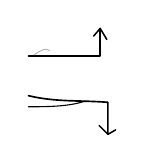
\begin{tikzpicture}[x=.014cm,y=-.014cm,line cap=round,line join=round]
\draw[line width=.55pt] (20,37)--(85,37)--(85,12);
\draw[line width=.55pt] (79,19)--(85,12)--(91,22);
\draw[gray!65,line width=.3pt] (25,36)..controls(31,32)and(36,29)..(39,32);
\draw[line width=.6pt] (20,73)..controls(45,79)and(68,77)..(92,79)--(92,108);
\draw[line width=.55pt] (84,100)--(92,108)--(99,104);
\draw[line width=.4pt] (20,83)..controls(36,83)and(56,83)..(71,78);
\end{tikzpicture}}&&&&&&\\[-.5ex]
\text{Découverte}&\text{Réveil}&\text{Die Eltern}&\text{Das Kind}&\text{Der Baumeister}&\text{Le Bâtisseur}&\\
\text{de la}&\text{en}&&&&&\\
\text{Méditation}&\text{\deleted{\unsure{C|Ca}}Cascades}&\text{(Les parents)}&\text{(L'enfant)}&\text{(Le Bâtisseur)}&&\\ \cline{1-6}
\deleted{(\unsure{\mathrm i})}&\deleted{(\unsure{\mathrm{ii}|\mathrm i})}&\deleted{(\unsure{\mathrm i|\mathrm{ii}})}&\deleted{(\unsure{\mathrm i|\mathrm{ii}})}&\deleted{(\unsure{\mathrm i|\mathrm{ii}})}&\deleted{(\unsure{\mathrm{ii}|\mathrm{iv}|\mathrm{iii}})}&\\
?\ \downarrow&\searrow&&&&&\text{\begin{tikzpicture}[x=1ex,y=1ex,line width=.28pt,line cap=round]\draw (.18,0)--(.68,.14)--(.07,.14);\end{tikzpicture}}\\
\deleted{\unsure{(\mathrm i)}}(\mathrm i)&(\mathrm{ii})&\deleted{\unsure{(}}(\mathrm i)&\deleted{(\mathrm i)}(\mathrm i)&(\mathrm i)&(\mathrm{iv})&\text{\begin{tikzpicture}[x=1ex,y=1ex,line width=.28pt,line cap=round]\draw (.10,0)--(.68,.14);\end{tikzpicture}}\\ \cline{1-6}
\text{Envol}&\text{Vers un plus long Voyage}&\text{Bild und Wahrheit}&\text{Der Wolf}&\text{Spiel- und Sucht}&\text{Le ``Maître''}&\text{\begin{tikzpicture}[x=1ex,y=1ex,line width=.28pt,line cap=round]\draw (.20,0)--(.60,.12);\end{tikzpicture}}\\
&&\text{(Image et Réalité)}&\text{(Le Loup)}&\text{(Jeu - et Fringale)}&&\\ \cline{1-6}
\text{M }1976\mathord{*}&\text{M }1979&\text{HS }\mathrm I&\text{Sch }\mathrm I&\text{Sch }\overline{\underline{\mathrm{VI}}}&\text{Sch }\overline{\underline{\mathrm{IX}}}&\text{\begin{tikzpicture}[x=1ex,y=1ex,line width=.28pt,line cap=round]\draw (.10,0)--(.50,.12);\end{tikzpicture}}
\end{array}\)}\endgroup}
% archive sheet number: 12

\scanpage{14}
\unsure{décompositions} \inserted{et découpages} $n$-aires d'\unsure{espaces} topologiques

% archive sheet number: 13

\scanpage{15}
\begingroup
\makeatletter
\tagsleft@true
\makeatother
\uline{\deleted{\unsure{I|V}}Version I}

Soient $X$ un espace topologique, $(\deleted{\unsure{\Sigma|S}}E_i)_{i\in I}$ un ens. de parties \inserted{\unsure{fermés|fermées}} de $X$ (noté indiciellement), telles que l'on ait
% slanted
\reversemarginpar
\margin{$\nearrow$ Supposons de plus que pour \unsure{tte|toute|tt} comp. conn. $\Sigma_{\unsure{i}}$ de $X\setminus E_i$, on ait $\overline{\Sigma}_i\cap E_i\ne\varnothing$ i.e. $\overline{\Sigma}_i\ne\Sigma_i$ i.e. $\Sigma_i$ non fermé dans $X$ (ce qui est le cas si $X$ est \unsure{d.} connexe)}
\normalmarginpar
\[
 \forall i\in I,\quad \operatorname{Card}\unsure{\pi_0|\Pi_0}(X\setminus\deleted{\Sigma}E_i)=2
 \tag*{(a)}
\]
\margin{\uline{NB} les comp. conn. $\Sigma_i^+,\Sigma_i^{\unsure{+|-|\ast}}$ de $X\setminus\Sigma_i$ sont ouvertes dans $X$}
\[
 \begin{aligned}
 &\forall(i,j)\in I\times I,\ i\ne j,\quad \deleted{\Sigma}E_j\ \text{est contenu dans l'une}\\
 &\text{des deux composantes connexes de }X\setminus\deleted{\Sigma}E_i.
 \end{aligned}
 \tag*{(b)}
\]

NB Cette condition (b) est vérifiée \unsure{automatiquement} les $\deleted{\Sigma}E_i$ $(i\in I)$ sont connexes, dès lors que les $E_i$ sont supposés disjoints mutuellement

On se propose d'étudier le ``découpage'' de $X$ par la famille $(E_i)$.

\uline{Cas $\operatorname{Card}\deleted{\unsure{(\mathrm{de})}}(I)\deleted{\unsure{\leq|=}}=2$}

Soit $\Sigma_i^+$ la comp. conn. de $X\setminus E_i$ qui ne contient pas $E_j$ $(j\ne i)$, alors on a (si $I=\{1,2\}$)
\figure{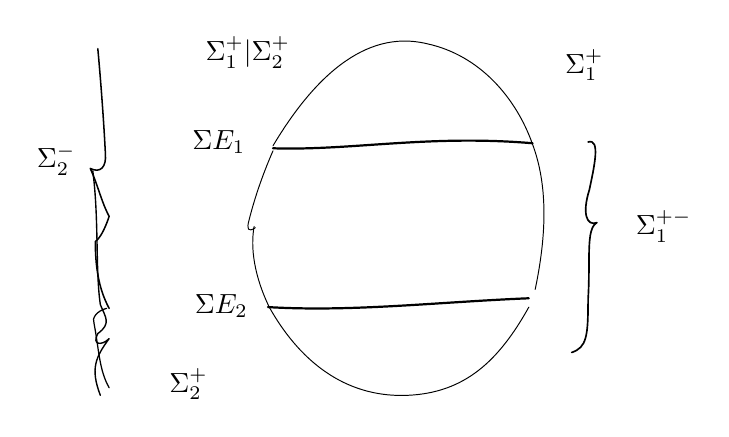
\begin{tikzpicture}[x=.016cm,y=-.016cm,line cap=round,line join=round]
\draw[line width=.35pt] (187,115) .. controls (218,63) and (259,22) .. (309,34)
 .. controls (351,43) and (380,77) .. (393,114)
 .. controls (403,141) and (406,177) .. (395,229);
\draw[line width=.35pt] (390,243) .. controls (366,286) and (339,311) .. (294,313)
 .. controls (249,315) and (211,291) .. (184,243)
 .. controls (172,218) and (169,196) .. (172,179);
\draw[line width=.35pt] (187,119) .. controls (180,135) and (173,154) .. (168,174)
 .. controls (166,181) and (167,184) .. (173,180);
\draw[line width=.8pt] (187,117) .. controls (249,119) and (310,106) .. (393,113);
\draw[line width=.8pt] (183,243) .. controls (250,247) and (317,239) .. (390,236);
\draw[line width=.55pt] (48,38) .. controls (51,71) and (53,101) .. (54,121)
 .. controls (55,132) and (50,137) .. (42,133)
 .. controls (48,146) and (51,160) .. (57,171)
 .. controls (53,183) and (49,189) .. (46,191)
 .. controls (46,215) and (50,231) .. (57,244);
\draw[line width=.5pt] (44,135) .. controls (49,173) and (46,214) .. (50,241)
 .. controls (54,251) and (59,256) .. (48,264)
 .. controls (43,273) and (51,274) .. (57,268)
 .. controls (46,283) and (42,292) .. (50,313);
\draw[line width=.45pt] (55,244) .. controls (47,246) and (43,252) .. (45,256)
 .. controls (49,277) and (49,293) .. (57,307);
\draw[line width=.6pt] (437,112) .. controls (447,109) and (442,131) .. (438,150)
 .. controls (432,169) and (436,179) .. (444,176)
 .. controls (435,181) and (439,205) .. (437,237)
 .. controls (437,266) and (436,275) .. (424,279);
\node at (167,41) {$\deleted{\unsure{\Sigma_1^+|\Sigma_2^+}}$};
\node at (144,112) {$\deleted{\unsure{\Sigma}}E_1$};
\node at (146,242) {$\deleted{\unsure{\Sigma}}E_2$};
\node at (434,51) {$\Sigma_1^+$};
\node at (497,179) {$\Sigma_1^{\deleted{\unsure{+}}\unsure{-}}$};
\node at (15,126) {$\Sigma_2^-$};
\node at (120,304) {$\Sigma_2^+$};
\end{tikzpicture}}
\[
 \Sigma_1^+\cap\Sigma_2^+=\varnothing
 \tag*{(1)}
\]
ce qui \deleted{résulte de}
\[
 \begin{aligned}
 &\deleted{\Sigma_1^-\supset\Sigma_2^+}\qquad\text{\unsure{équivaut à|équiv. à :}}\\
 &\deleted{\Sigma_2^-\supset\Sigma_1^+}\qquad \Sigma_1^+\subset\Sigma_2^-\cup E_2,\quad\text{et}
 \end{aligned}
\]
(\deleted{\unsure{car si}} \deleted{Si on avait} comme $\Sigma_1^+\cap E_2=\varnothing$, cela équivaut aussi à
\[
 \Sigma_1^+\subset\Sigma_2^-
 \tag*{(2)}
\]
\unsure{et} symétriquement, à
\[
 \Sigma_2^+\subset\Sigma_1^-
 \tag*{$(2')$}
\]

Comme \deleted{\unsure{vois. ouvert}} $\Sigma_2^-\supset E_1$, \deleted{il contient les} \inserted{i.e. $\Sigma_2^-$ est un \uline{vois.} ouvert de $E_1$,} on a
% slanted
\reversemarginpar
\margin{$\overline{\Sigma_1^+}\cap E_1\ne\varnothing$ i.e. $\overline{\Sigma_1^+}\ne\Sigma_1^+$ \unsure{à sign.ler|à signaler} avant}
\normalmarginpar
\[
 \Sigma_2^-\cap\Sigma_1^+\ne\varnothing
\]
Car $\underline{\overline{\Sigma_1^+}\cap E_1}\ne\varnothing$ (sinon \inserted{l'ouvert} $\Sigma_1^+$ serait \inserted{\unsure{un|une}} fermé dans $X$, \unsure{puis|donc} \deleted{\unsure{\Sigma_1^+\ne\varnothing|\Sigma_1^+\text{ serait}}} $X$ serait disconnexe),
\endgroup
% archive sheet number: 14

\scanpage{16}
et par suite $\Sigma_2^-\cup\Sigma_{\deleted{\unsure{2}}1}^+$ \deleted{\unsure{sera|sont}} est un ouvert connexe de $X$ donc de $X\setminus E_2$, contenant \inserted{la comp. conn.} $\Sigma_2^-$ \inserted{de $X\unsure{/|\setminus}E_{\unsure{2}}$}, donc \deleted{\unsure{c'est}} \unsure{égale|égal} \unsure{:|à} $\Sigma_2^-$, \unsure{donc|d'où} $\Sigma_1^+\subset\Sigma_2^-$, \unsure{cqfd|qfd}

L'intersection des deux partitions
\[
 \begin{aligned}
 X&=\deleted{\unsure{E}}\Sigma_1^+\amalg E_1\amalg\Sigma_1^-\\
 X&=\Sigma_2^+\amalg E_2\amalg\Sigma_2^-
 \end{aligned}
\]
de $X$ est
\[
 X=\overbrace{\Sigma_1^+\amalg E_1\amalg
 \rlap{$\displaystyle\underbrace{\phantom{E\Sigma_{12}}\amalg
 E_2\amalg\Sigma_2^+}_{\Sigma_1^-}$}\deleted{E}\Sigma_{12}}^{\Sigma_2^-}
 \phantom{\amalg E_2\amalg\Sigma_2^+}
\]
avec
\[
 \Sigma_{12}\overset{\text{def}}{=}\Sigma_1^-\cap\Sigma_2^-
\]

\deleted{\unsure{O}}Dans cette partition, $\Sigma_1^+,\Sigma_{12},\Sigma_2^+$ sont ouverts $E_1,E_2$ sont fermés, et on a
\[
 \begin{aligned}
 &\Sigma_1^+\subsetneq\overline{\Sigma_1^+}\subset\Sigma_1^+\cup E_1\\
 &\overline{\Sigma_{12}}\subset\overline{\Sigma_1^-}\cap\overline{\Sigma_2^-}\subset
 (\Sigma_1^-\cup E_1)\cap(\Sigma_2^-\cup E_2)\subset\Sigma_{12}\cup E_1\cup E_2\\
 &\Sigma_2^+\subsetneq\overline{\Sigma_2^+}\subset\Sigma_2^+\cup E_2
 \end{aligned}
\]

Notons aussi que
\[
 \overline{\Sigma_{12}}\cap E_1\ne\varnothing,\quad
 \overline{\Sigma_{12}}\cap E_2\ne\varnothing
\]
Car si on avait p.\,ex. $\overline{\deleted{\unsure{E}}\Sigma_{12}}\cap
\deleted{\unsure{\Sigma}}E_1=\varnothing$, on \deleted{alors $\Sigma_{12}\amalg E_2\amalg\Sigma_2$}
\inserted{en conclurait} $\overline{\Sigma_1^-}\cap E_1=\varnothing$,
\[
 \begin{aligned}
 \big[\,\text{car}\quad\overline{\Sigma_1^-}&=
 \overline{\Sigma_2^+\deleted{\unsure{\amalg}}\cup E_2
 \deleted{\unsure{\amalg}}\cup\Sigma_{12}}=
 \underbrace{\overline{\Sigma_2^+}}_{\subset\,\Sigma_2^+\cup E_2}\cup E_2
 \cup\overline{\Sigma_{12}}\subset\Sigma_1^-\cup\overline{\Sigma_{12}}\unsure{\big]}
 \end{aligned}
\]
ce qui n'est pas.

% archive sheet number: 15

\scanpage{17}
\uline{Cas particuliers}

Supposons que $\forall i\in I$, \deleted{$E_i$ \unsure{soit|est} \unsure{rare|dense} dans $X$.} \inserted{on ait} (si $\Sigma_i^+\ \Sigma_i^-$ sont les deux comp. conn. de $X\setminus\Sigma_i$)

\deleted{Alors on \unsure{trouve} que}
\[
\begin{aligned}
\overline{\Sigma_i^+} &= \Sigma_i^+\cup E_i\\
\overline{\Sigma_i^-} &= \Sigma_i^-\cup E_i .
\end{aligned}
\]

Alors je dis qu'on a
\[
\overline{\Sigma_{12}}=\Sigma_{12}\cup E_1\cup E_2
\]

\noindent\rule{2.4cm}{0.3pt}\par

% slanted
\reversemarginpar
\margin{\unsure{introduire|introduisons} la partition $\Pi_j=\{\deleted{\unsure{\Sigma}}E_j,\Sigma_j^+,\Sigma_j^-\}$}
\normalmarginpar
\deleted{Supposons}

Soit $J\subset I$ tel que $I=J\amalg\{i\}$.

Considérons la partition \inserted{$\Pi_J$} de $X$ \deleted{\unsure{définie|définies|des parties}} définie par les $\deleted{\unsure{\Sigma}}E_j$ $(j\in J)$, \deleted{\unsure{et}} \unsure{intersection} des partitions \inserted{ternaires $\Pi_j$} de $X$ $(j\in J)$ définies par les $E_j$ \deleted{$\unsure{E|\in}$} $(j\in J)$
\[
X=E_j\amalg\coprod_{\alpha\in\pi_0(X\setminus E_j)}\Sigma_j^\alpha
\]

-- c'est aussi la partition définie par celle de $\displaystyle\bigcup_{j\in J}E_j$ en les $E_j$, et la partition \inserted{$\Pi_J^{\unsure{\circ|0}}$} de $\displaystyle X\setminus\mathop{\overline{\bigcup}}\limits_{j\in J}E_j$ intersection des partitions binaires $\Pi_{J,j}^{\circ}$ \inserted{$(j\in J)$} \unsure{induites|déduites} sur \inserted{$U_{\deleted{\unsure{J|j}}J}={}$} $\displaystyle X\setminus\bigcup_{j\in J}E_j$ par les $\Pi_j$ $(\unsure{g|j}\in J)$. P. \unsure{ex}
% archive sheet number: 16

\scanpage{18}
cette dernière, si $\operatorname{card}J=\operatorname{card}I-1=n-1$, on verra (par récurrence) que le cardinal de l'ens des classes est $(n-1)+1=n$.

Ceci posé, on voit d'abord que $E_i$ est dans l'une \inserted{(unique)} \unsure{de|des} ces $n$ classes, qui sont des ouverts. Soit $U_{J,i}$ la classe (ou ``composante'') qui contient $E_i$, et considérons les deux composantes $\Sigma_i^+,\Sigma_i^-$ de $X\setminus E_i$.

\noindent\begin{tabular}{@{}|p{.91\linewidth}@{}}
\uline{Lemme} Toute classe de $\Pi_{J\deleted{\unsure{i|j|,}}}^{\unsure{\circ|0}}$, distincte de $U_{J,i}$, est contenue dans $\Sigma_i^+$ ou $\Sigma_i^-$
\end{tabular}

C'est presque une tautologie : Dire \deleted{la} \inserted{qu'une} classe donnée \inserted{$U_{\unsure{\alpha|x}}$\unsure{,} de $\Pi_J^\circ$} ne contient pas $\deleted{\unsure{\Sigma}}\unsure{\overline{E_i}|E_i}$ i.e. est $\ne U_{J,i}$, signifie que il existe un $j\in J$ tel que le $\Sigma_j^+\in\pi_0(X\setminus \deleted{\unsure{\Sigma}}E_j)$ \deleted{\unsure{choisi|choisie}} ``\unsure{composant|composante}'' de cette classe \deleted{est} est l'élément du $\pi_{\unsure{0}}$ qui ne contient pas $E_i$; il est donc contenu dans l'un des éléments \inserted{(soit $\Sigma_i^-$)} de $\pi_0(X\setminus\unsure{\Sigma_i|\overline{\Sigma_i}})$, d'après l'étude du cas \deleted{\unsure{deux}} \inserted{$\operatorname{card}I=2$}, \deleted{\unsure{OK|cela|elle}} \unsure{â|à} fortiori $U_\alpha\subset\Sigma_i^-$, OK.
% archive sheet number: 17

\scanpage{19}
Dém. par récurrence, c'est trivial si $\operatorname{card} I=0,1$ Le cas $\operatorname{card} I=2$ \unsure{a} été vu. Cas général \unsure{avec} $\operatorname{card} I\geq 3$, on choisit $J$ comme dessus. Il suffit de voir que les ens.
\[
\unsure{U|\deleted{=}U}_{J,i}\cap\Sigma_i^+,\ U_{J,i}\cap\Sigma_i^-
\]
ont la forme précédente, il suffit de le voir pour \unsure{l'une|l'un} des deux.

Par hyp. de récurrence, \unsure{on a}
\[
U_{J,i}=X\setminus\coprod_{\alpha\in \deleted{\unsure{J}}K_0}\widehat{\Sigma}_\alpha^+
\]
où
\[
\left\{\begin{aligned}
&\deleted{\Sigma_{\unsure{\alpha|0}}}K_0\subset J\\
&\Sigma_\alpha^+\in\unsure{\pi_0|\Pi_0}(X\setminus E_\alpha)\qquad (\forall\,\alpha\in K_0)\\
&\widehat{\Sigma}_\alpha^+=\Sigma_\alpha^+\cup E_\alpha.
\end{aligned}\right.
\]
\deleted{\unsure{D|O}}\unsure{On a} donc
\[
U=U_{J,i}\cap\Sigma_i^-=X\setminus\left(\coprod_{\alpha\in K_0}\widehat{\Sigma}_\alpha^+\ \cup\ \widehat{\Sigma}_i^+\right)
\]
\deleted{Soit} Au deuxième $=$, dans la \deleted{\unsure{somme|réunion}} réunion $\bigcup_{\alpha\in K_0}\widehat{\Sigma}_\alpha^+$, il suffit de se borner \unsure{à|:} \unsure{sommer} sur les \deleted{$\Sigma$} $\alpha\in K_0$ tels que $\widehat{\Sigma}_\alpha^+\not\subset\widehat{\Sigma}_i^+$ i.e. $\Sigma_\alpha^+\not\subset\Sigma_i^+$ soit $K_1$ cet ens., donc
\[
U=X\setminus\left(\bigcup_{\alpha\in K_1}\widehat{\Sigma}_\alpha^+\ \cup\ \widehat{\Sigma}_i^+\right)
\]
% archive sheet number: 18

\scanpage{20}
Ainsi les classes de $\Pi_I^{\unsure{\circ|0}}$ sont les classes de $\Pi_J^\circ$ distinctes de $\deleted{\Pi}U_{J,i}$, et de plus les \unsure{clas.|deux.} parmi
\[
U_{J,i}\cap\Sigma_{\unsure{\deleted{J}i|j|i}}^+,\ U_{J,i}\cap\Sigma_i^-
\]
qui sont non vides. Or les deux classes en question sont non vides, car \deleted{$\unsure{\Sigma_i|\Sigma_j}$} $U_{J,i}$ est un voisinage de $\deleted{\Sigma}E_i$, et
\[
\overline{\Sigma_i^+}\cap\deleted{\Sigma}E_i\ne\varnothing,\quad
\overline{\deleted{\unsure{E}}\Sigma_i^-}\cap\deleted{\Sigma}E_i\ne\varnothing.
\]
On \unsure{sait|voit} donc que le nb des classes est en \deleted{\unsure{tout|est}} $(n-1)+2=n+1=\operatorname{card} I+1$ (ce qui achève \unsure{aussi|ainsi} la dém. par récurrence sur le nb des classes).

\uline{Lemme} Toute classe de $\Pi_I^\circ$ est de la forme $X\setminus\bigcup_{\alpha\in\deleted{I}K}(\overbrace{\Sigma_\alpha^+\cup E_\alpha}^{\inserted{\widehat{\Sigma}_\alpha^+}})$ où $K$ est une partie \inserted{\deleted{non vide}} de $I$, et
% slanted
\reversemarginpar\margin{\shortstack[l]{$K$ est $\ne\varnothing$\\si $I\ne\varnothing$}}\normalmarginpar
$\forall\alpha\in K$, \deleted{on a} $\Sigma_\alpha^+\deleted{\unsure{\Rightarrow|\to}}\in\pi_0(X\setminus E_\alpha)$, tels que $\forall\alpha,\beta\in K$, $\alpha\ne\beta$, on ait $\widehat{\Sigma}_\alpha^+\cap\widehat{\Sigma}_\beta^+=\varnothing$ $(\Longleftrightarrow\Sigma_\alpha^+\cap\Sigma_\beta^+=\varnothing)$.
% archive sheet number: 19

\scanpage{21}
Soit $\alpha_0\in K_1$, je dis que \unsure{l'on a|on a}
\[
\widehat{\Sigma}_{\alpha_0}\cap\widehat{\Sigma}_i^+=\varnothing
\qquad\text{i.e}\qquad
\Sigma_{\alpha_0}\cap\Sigma_i=\varnothing
\]
(ce qui achèvera la démonstration, car on aura
\[
U=X\setminus\bigcup_{\alpha\in K}\widehat{\Sigma}_\alpha^+
\qquad\left\{\begin{aligned}
&K=K_1\cup\{i\}\\
&\deleted{\unsure{\Sigma_\alpha}}
\end{aligned}\right.
\]
comme dans le lemme.

Or \unsure{comme} on a
\[
E_i\subset U_{J,i}=X\setminus\mathop{\rlap{\raisebox{.65ex}{$\scriptstyle-$}}\bigcup}\limits_{\alpha\in K_0}\widehat{\Sigma}_\alpha^+
\]
cela implique que
\[
E_i\subset X\setminus\widehat{\Sigma}_{\alpha_0}^+=\Sigma_{\unsure{\alpha_0|\alpha}}^-
\]
% margin note written sideways
\margin{\unsure{j:e.|j.e.|i.e.}\diagram{\begin{tikzcd}[ampersand replacement=\&,column sep=0pt,row sep=0.9ex,execute at end picture={
\draw ([xshift=-4.0mm]dTop.west) .. controls +(0.7mm,-1mm) and +(1mm,2mm) .. ([xshift=-4.1mm]dMid.west) .. controls +(-1mm,-.8mm) and +(1mm,.5mm) .. ([xshift=-5mm]dMid.west) .. controls +(1mm,-.5mm) and +(1mm,.8mm) .. ([xshift=-4.1mm,yshift=-1mm]dMid.west) .. controls +(.5mm,-2mm) and +(-.6mm,1mm) .. ([xshift=-4.6mm]dEnd.west);
\draw ([xshift=-.9mm]dMid.west) .. controls +(-.4mm,-1mm) and +(.9mm,.7mm) .. ([xshift=-1.1mm]dE.west) .. controls +(-1mm,-.4mm) and +(.7mm,.1mm) .. ([xshift=-1.8mm]dE.west) .. controls +(.7mm,-.1mm) and +(.8mm,.5mm) .. ([xshift=-1.1mm,yshift=-.5mm]dE.west) .. controls +(.4mm,-1mm) and +(-.5mm,.6mm) .. ([xshift=-.8mm]dEnd.west);
\node[rotate=90,inner sep=0pt] at ([xshift=-2.7mm,yshift=-1mm]dE.west) {$\scriptscriptstyle\Sigma_i^-\,\unsure{\rotatebox{-90}{$!$}|\text{ou}|-}\,\Sigma_i^+$};
}]
|[alias=dTop,anchor=west]| \scriptstyle\Sigma_i^+\ \text{ou}\ \Sigma_i^-\\
|[anchor=west]| \scriptstyle E_i\\
|[alias=dMid,anchor=west]| \scriptstyle\Sigma_{i\alpha}\\
|[alias=dE,anchor=west]| \scriptstyle E_\alpha\\
|[alias=dEnd,anchor=west]| \scriptstyle\Sigma_{\alpha_0}^+
\end{tikzcd}}}
d'autre part $\alpha_0\in K_1$ \unsure{signifi|signifie}
\[
\Sigma_{\alpha_0}^+\not\subset\Sigma_i^+
\]
ce qui \deleted{\unsure{impli|impl.}} signifie aussi que $\Sigma_i^+\cap\Sigma_\alpha^+=\varnothing$, cqfd.

\uline{Corollaire du lemme} Pour une classe

\noindent\begin{tabular}{@{}|p{.96\linewidth}@{}}
$V$ de $\Pi_I^{\unsure{\circ|0}}$, son expression
\[
V=X\setminus\bigcup_{\alpha\in K}\widehat{\Sigma}_\alpha^+
\]
du lemme précédent est \uline{unique} -- on a
{\small
\[
\left\{\begin{aligned}
&K=\{\alpha\in I\mid\overline V\cap E_\alpha\ne\varnothing\quad\text{i.e.}\quad\deleted{V}E_\alpha\cap\dot V\ne\varnothing\}\\
&\Sigma_\alpha^+\ \text{est l'unique comp. de }X\setminus\Sigma_\alpha\ \text{contenue dans }X\setminus V
\end{aligned}\right.
\]}
\end{tabular}
% archive sheet number: 20

\scanpage{22}
\deleted{\unsure{On|Un} procède par récurrence sur $\operatorname{card} K$,} \inserted{On note d'abord que} \deleted{pour prouver que} (si $V=\underset{\substack{\rotatebox{90}{$=$}\\ \inserted{\bigcap_{\alpha\in K}\Sigma_\alpha^-}}}{\underbrace{X\setminus\bigcup_{\alpha\in K}\widehat{\Sigma}_\alpha^+}}$, les $\widehat{\Sigma}_\alpha^+$ \unsure{(}$\alpha\in K$\unsure{)} étant \unsure{disjoints|disjointes})
\[
\left\{\begin{aligned}
&\overline V\cap E_\alpha\ne\varnothing\\
&\makebox[0pt][r]{$\longrightarrow$\hspace{.15em}}V\cap\Sigma_\alpha^-\deleted{\unsure{\ne|=}\varnothing}\ne\varnothing
\qquad\text{alors que } V\cap\Sigma_\alpha^+=\varnothing
\end{aligned}\right.
\]
\reversemarginpar\margin{\raggedleft\raisebox{.8\baselineskip}{trivial}}\normalmarginpar

De façon précise, je dis que
\[
\begin{array}{ccc@{\quad}l}
\overline V\cap E_\alpha & = & \overline{\Sigma_\alpha^-}\cap E_\alpha & \text{(qui est donc }\ne\varnothing\text{)}\\[-2pt]
\rotatebox{90}{$=$} && \rotatebox{90}{$\unsure{\deleted{=}|=}$} &\\[-2pt]
\inserted{\overline V\cap\widehat{\Sigma}_\alpha^+} && \inserted{\overline{\Sigma_\alpha^-}\cap\widehat{\Sigma}_\alpha^+} &
\end{array}
\]

\deleted{Comme $V\subset\Sigma_\alpha^-$, on a $V\cap E_\alpha\subset\overline{\Sigma_\alpha^-}\cap E_\alpha$, prouvons l'inclusion inverse}
\[
\deleted{\overline{\Sigma_\alpha^-}\cap E_\alpha\subset\overline V\cap E_\alpha}
\]
\deleted{Soit $x\in\overline{\Sigma_\alpha^-}\cap E_\alpha$, prouvons $x\in\overline V\cap E_\alpha$ i.e.} \deleted{$x\in\overline V$, soit $W$ un voisinage de $x$, montrons qu'il} \deleted{rencontre}

\deleted{Or} \deleted{\unsure{on}} \deleted{peut considérer cette} \deleted{\unsure{formule}} \deleted{\inserted{égalité}} \deleted{comme égalité dans} \deleted{l'espace}
\[
\deleted{\unsure{Y|\deleted{Z}Y|Z|X}=\widehat{\Sigma}_\alpha^-=\Sigma_\alpha^-\cup E_\alpha}
\]
\deleted{dans lequel on a deux parties fermées} \deleted{disjointes}

Or dans $X$ on a les deux parties \uline{fermées} \uline{disjointes}
\[
Y=\widehat{\Sigma}_\alpha^+,\qquad Z=\bigcup_{\beta\in K\setminus\{\alpha\}}\widehat{\Sigma}_\beta^+
\]
et on doit prouver
\[
\overline{(X\setminus(Y\cup Z))}\cap Y=\overline{(X\setminus Y)}\cap Y
\]
ce qui est immédiat
% archive sheet number: 21

\scanpage{23}
Soit maintenant $\beta\in I\setminus K$, prouvons que l'on a $\overline V\cap E_\beta=\varnothing$. En effet, $V$ ne \deleted{contient} \inserted{rencontre} aucun $E_i$ $(i\in I)$ donc $E_\beta\subset X\setminus V=\mathop{\unsure{\deleted{\bigvee}\bigcup|\bigcup}}\limits_{\alpha\in K}\widehat{\deleted{\unsure{I|E}}\Sigma}_\alpha^+$, \deleted{\unsure{donc si}} je dis que si $\beta\in I\setminus K$, on a en fait
\[
E_\beta\subset\bigcup\Sigma_\alpha^+\qquad\text{(ouvert disjoint de }V\text{)}
\]
% slanted
\reversemarginpar\margin{\makebox[\linewidth][r]{\rotatebox{24}{\shortstack[l]{C'est trivial, \deleted{\illegible{1}}\\du fait que les $E_i$ $(i\in\unsure{I|J})$\\sont disjoints}}}}\normalmarginpar
ce qui \unsure{prouvera|prouve} l'assertion -- mieux, je dis que $\exists\alpha\in K$ tel que $E_\beta\subset\Sigma_\alpha^+$. Cela \unsure{revient|mérite} \unsure{au|un}

\uline{Lemme} Soit $K\subset I$, \deleted{tel que les} \deleted{et} des $\Sigma_\alpha^+$ $(\alpha\in K)$ tels que
\[
\alpha\mathrel{\unsure{\ne|\deleted{\ne}{,}}}\beta\in K,\ \alpha\ne\beta\ \Rightarrow\ \Sigma_\alpha^+\cap\Sigma_\beta^+=\varnothing.
\]
Soit $i\in I\setminus K$ tel que $E_i\subset\bigcup\Sigma_\alpha^+$, alors \deleted{$E_i$ est \unsure{contenu|contenue}} \inserted{$\exists\alpha\in K$ tel que} $E_i\subset\Sigma_\alpha^+$.

\unsure{Ce $L^\circ$|Ce $L^o$|Cela} \deleted{signifie que} \unsure{provient|précise|précise le} \unsure{du|des|sens|donc}

\uline{Corollaire} Avec les hyp. préc. sur $(\Sigma_i^\alpha)_{\alpha\in\unsure{K|I}}$,

\noindent\begin{tabular}{@{}|p{.96\linewidth}@{}}
la partition $\Pi_K^{\unsure{\circ|0}}$ est formée des $\Sigma_\alpha^+$ $(\alpha\in K)$ et de $V=X\setminus\mathop{\overline{\bigcup}}\limits_{\alpha\in K}\widehat{\Sigma}_\alpha^+$.
\end{tabular}

Immédiat par récurrence sur $\operatorname{card} K\geq 0$.
% archive sheet number: 22

\scanpage{24}
Considérons la partition $\Pi_I^{\unsure{\circ|0}}$ de $X\setminus\bigcup_{\alpha'\in I}E_{\alpha'}$, soit $S$ l'ens des classes, notées $U_s$ $(s\in S)$. \deleted{\unsure{On a|On}} Considérons la \deleted{\uline{Lemme} $\forall i\in I$,} \inserted{Relation $R$ entre $S$ et $I$}
\[
\deleted{\unsure{U|E}}(s,i)\in R\ \overset{\text{def}}{\Longleftrightarrow}\ \overline{U_s}\cap E_i\ne\varnothing.
\]

\uline{Lemme} Cette relation fait de $(S,I\unsure{)\deleted{R})|\deleted{)}{,}R)}$

\noindent\begin{tabular}{@{}|p{.94\linewidth}@{}}
un graphe strict ayant $S$ comme \unsure{ens des|ens de} sommets, $I$ comme ens. \unsure{de|d'} \unsure{arêtes|arètes|aretes}.) \deleted{Cette relation} \unsure{Le|Ce} graphe est un \uline{arbre}
\end{tabular}

le fait qu'on a un graphe strict signifie que a) $\forall i\in I$, Il \deleted{\unsure{existe|ex}} y a exactement deux $U_s$ tels que $\overline{U_s}\cap E_i\ne\varnothing$, et b) $i$ est caractérisé par l'ens de ces deux $U_s$.

\unsure{Soient|Soit} $\Sigma_i^+,\Sigma_i^-$ les deux comp. \unsure{connexes} de $X\setminus E_i$, alors a) se précise en : il y a \unsure{exactement|exactemt|existe} \uline{un} $U_{s_{\unsure{+|-}}}$ contenu dans $\Sigma_i^{\unsure{+|-}}$ tel que $\overline{U_{s_{\unsure{+|-}}}}\cap E_i\ne\varnothing$ (et de $=$ pour $\Sigma_i^-$, \unsure{dé|qui} \unsure{définit|definit} un $U_{s_-}\subset\Sigma_i^-$ tel que $\overline{U_{s_-}}\cap E_i\ne\varnothing$),
% archive sheet number: 23

\scanpage{25}
\deleted{Soit en effet} Si on a $U_s\subset\deleted{\unsure{E|I}}\Sigma_i^-$, $\overline{U_s}\deleted{=}\cap E_{\unsure{i|j}}\ne\varnothing$, \deleted{et si} alors \unsure{on a}
\[
\begin{aligned}
U_s=X\setminus\mathop{\unsure{\rlap{\raisebox{.65ex}{$\scriptstyle-$}}\bigcup|\deleted{\bigcap}\bigcup}}\limits_{\alpha\in K}\widehat{\Sigma}_\alpha^+
&\qquad\text{où}\quad i\in K\subset I\\
&\forall\alpha\in K\qquad\Sigma_\alpha^+\in\pi_0(X\setminus E_\alpha)\ \deleted{\unsure{\text{les}|K|\text{tel}|\text{et}}}\\
&\deleted{\unsure{U\Sigma|\bigcup\Sigma|U}}\ \text{les }\Sigma_\alpha^+\ \text{mut\textsuperscript{t}. \unsure{disjoints}}
\end{aligned}
\]
Il faut voir que $\deleted{K}\inserted{K\setminus\{i\}}$ et les $\Sigma_\alpha^+$ $(\alpha\in K\setminus\{i\})$ sont determinés en termes de $i$ et de $\Sigma_i^+$ i.e. $\Sigma_i^-$. Je dis que
\[
K\setminus\{i\}=\bigl\{\alpha\in I\mid E_\alpha\subset\Sigma_\alpha^-
\]
% archive sheet number: 24

\scanpage{26}
Soit $X$ un ens. Une \uline{décomposition binaire} de $X$ est un ens de deux parties de $X$ $(\Sigma_{\alpha}^{\alpha})_{\alpha\in\unsure{\mathcal E|\mathscr E|\varepsilon}}$ (les ``hémisphères'') dont la réunion est $X$, et dont \deleted{l'intersection} aucune n'est contenue dans l'autre -- on désigne par $E$ (``équateur'') l'intersection (on n'exclut pas qu'elle soit vide). Quand $X$ est un espace topologique, on s'intéresse au cas où les hémisphères $\Sigma_{\alpha}$ sont fermés, (et \inserted{de} plus, le plus souvent, \inserted{$\Sigma_{\alpha}^{\alpha}$ et $\Sigma_{\deleted{\unsure{\alpha}}}^{\alpha}\setminus E=\Sigma_{\deleted{\unsure{\alpha}}}^{\deleted{\unsure{\alpha}}\alpha,\unsure{0|\circ|o}}$} connexes \deleted{\unsure{$\Sigma_{\alpha}$|les}} et où $E\ne\varnothing$); si les $\Sigma_{\deleted{\unsure{\alpha}}}^{\alpha}$ connexes et $E\mathrel{\unsure{\ne|+}}\varnothing$, $X$ est connexe, si \deleted{les $\Sigma_{\alpha}^{\alpha,0}$ connexes}, \inserted{$X$ connexe, \deleted{et}} on conclut \unsure{\deleted{aussitôt}} que $\overline{\Sigma^{\alpha,0}}\cap E\ne\varnothing$
% margin note written sideways
\reversemarginpar\margin{\figure{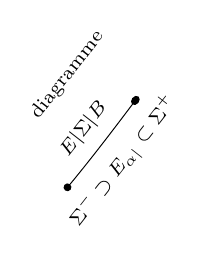
\begin{tikzpicture}[x=1mm,y=1mm,line cap=round,line join=round,font=\scriptsize]
\begin{scope}[rotate=52,transform shape]
\draw[line width=.35pt] (0,0) .. controls (4.6,-.15) and (9.5,-.08) .. (14,0);
\fill (0,0) circle[radius=.5mm];
\fill (14,0) ellipse[x radius=.64mm,y radius=.49mm];
\node[anchor=base west,inner sep=0pt] at (4.4,8.2) {diagramme};
\node[inner sep=0pt] at (7.1,2.9) {$\deleted{\unsure{E|\Sigma|B}}$};
\node[inner sep=0pt] at (7,-3.6) {$\Sigma^{-}\supset E_{\unsure{\alpha|{}}}\subset\Sigma^{+}$};
\end{scope}
\end{tikzpicture}}}\normalmarginpar
(car $\overline{\Sigma^{\alpha,0}}\cap E=\overline{\Sigma^{\alpha,0}}\setminus\Sigma^{\alpha,0}$, et $\Sigma^{\alpha,0}$ ne peut être à la fois ouvert et fermé car $\Sigma^{\unsure{-,0|\alpha,0|-\alpha,0}}$, est un ouvert $\ne\varnothing$ et $\ne X$)

Considérons deux décompositions binaires $\{\Sigma_1^{+},\Sigma_1^{-}\},\unsure{[|(}\Sigma_2^{+},\Sigma_2^{-}\}$ \deleted{\unsure{distinctes}} \inserted{de $X$,} on dit qu'elles sont \uline{\unsure{non panachées|non penchées|non parallèles|en position}} si \inserted{elles sont \uline{distinctes}, et si} on peut trouver $\Sigma_1^{+}$ dans l'une, $\Sigma_2^{+}$ dans l'autre, tels que
\[
\Sigma_1^{+}\cap\Sigma_2^{+}=\varnothing\qquad(\text{d'où }E_1\cap E_2=\varnothing)
\]
on \unsure{a} alors
\[
\begin{aligned}
\Sigma_1^{+}&\mathrel{\unsure{\deleted{\cap}\subset|\subset}}\Sigma_2^{-}\ \deleted{\ne\varnothing}\quad\text{i.e.}\quad\Sigma_1^{+}\cap\Sigma_2^{-}=\Sigma_1^{+}\\
\Sigma_2^{+}&\subset\Sigma_1^{-}\qquad\qquad\text{\unsure{i.e.|ie}}\quad\Sigma_2^{+}\cap\Sigma_1^{-}=\Sigma_2^{+}\\
\Sigma_{12}&\overset{\text{déf}}{=}\Sigma_1^{-}\cap\Sigma_2^{-}\supset E_1\cup E_2,\quad\Sigma_1^{-}\cap\Sigma_2^{-}\ne\varnothing
\end{aligned}
\]
% archive sheet number: 25
